\documentclass[../main.tex]{memoir}

\begin{document}

\chapter{Experimentación y resultados obtenidos}
\label{sec:experiments-and-results}

En este capítulo describiremos la experimentación realizada, así como
los resultados obtenidos. Comenzaremos describiendo los aspectos de
implementación y las bibliotecas utilizadas. Después, pasaremos a
comentar cómo hemos repetido la experimentación original del artículo,
y finalmente la experimentación de nuestra propuesta.

\section{Aspectos de implementación}

La implementación del trabajo ha sido realizada en Python 3.6. El
código desarrollado para el trabajo, el cual permite replicar la
experimentación llevada a cabo, se encuentra disponible en el
repositorio \url{https://github.com/fluque1995/tfm-anomaly-detection}.
Se proporcionan los modelos preentrenados para el experimento en el
que se utiliza una representación de tamaño 1024. El resto de
modelos no se han proporcionado porque la experimentación es similar
en todos los casos, y hemos preferido incluir sólamente el mejor
de los modelos.\\

Se utiliza como base para la implementación original el código
localizado en
\url{https://github.com/ptirupat/AnomalyDetection_CVPR18}. En dicho
repositorio se ofrece una implementación del modelo, así como el
archivo comprimido de la arquitectura original entrenada. No obstante,
no está disponible el código necesario para entrenar de nuevo el
sistema. Además, el autor del artículo ofrece el código en
\url{https://github.com/WaqasSultani/AnomalyDetectionCVPR2018}.\\

Para que la comparación entre nuestro modelo y el original fuese más
justa, se ha optado por repetir la experimentación llevada a cabo por
los autores, para evitar así posibles diferencias en el entrenamiento
de los modelos. Esto se debe a que no podemos garantizar que estamos
ejecutando exactamente los mismos pasos que los autores originales a
partir del código que proporcionan, ya que no está completo. Por
ejemplo, en ninguno de los dos repositorios se proporciona el código
para la extracción de características, así que no podemos asegurar que
los resultados que obtenga el modelo original a partir de las
características extraídas por nosotros sean idénticos a los que se
obtuvieron originalmente. A pesar de ello, incluimos también sus
resultados, los cuales muestran que el modelo entrenado por nosotros
no tiene exactamente el mismo comportamiento que el suyo.\\

De esta manera, tendremos dos versiones del modelo original, una
basada en el modelo entrenado que ofrecen los autores, y otra
entrenada completamente por nosotros. En cuanto a la implementación y
entrenamiento completos del modelo original, se han utilizado las dos
fuentes anteriores para replicar la experimentación de la forma más
fiable posible. No obstante, debido a que había gran parte del código
replicado entre ambos repositorios, y algunas partes estaban
implementadas de forma poco eficiente, se han realizado algunos
cambios en partes del código respetando su funcionamiento original. No
se ha utilizado directamente el código original del artículo por la
imposibilidad de replicar algunas de las etapas. Por ejemplo, hay
partes del sistema escritas en MATLAB, o que necesitan del uso de
herramientas externas. La implementación que hemos realizado permite
repetir por completo la experimentación utilizando Python
exclusivamente, y sin necesidad de recurrir a fuentes externas.\\

Para el tratamiento de los datos en formato de vídeo se ha utilizado
la librería OpenCV \cite{bradski2000opencv}. OpenCV es una librería de
código abierto pensada para el desarrollo de aplicaciones que se basan
en la visión por computador. En particular, hemos utilizado los
módulos que permiten la lectura de vídeos desde disco a memoria. Esta
librería carga los vídeos como una lista de matrices numéricas, las
cuales representan cada uno de los fotogramas que componen la
secuencia de vídeo. Para el manejo de dichas matrices, hemos hecho uso
de la librería de cálculo numérico NumPy \cite{oliphant2006guide,
  van2011numpy}. Este paquete ofrece una interfaz para operar de forma
eficiente con colecciones estructuradas de números
(\textit{N-dimensional arrays}). Debido a que Python es un lenguaje
orientado a la flexibilidad y la facilidad de uso, tiene como
contrapartida una pérdida importante de rendimiento cuando se realizan
operaciones aritméticas. Por este motivo, NumPy resulta ser una
herramienta fundamental para el desarrollo de aplicaciones con alto
coste computacional. Además, para la gestión efectiva de los archivos
de anotaciones, los cuales se proporcionan en formato CSV, se ha hecho
uso de Pandas \cite{reback2020pandas}. Esta librería permite el manejo
de datos estructurados en tablas, utilizando para ello estructuras
conocidas como \textit{DataFrames}.\\

Para la implementación de los modelos de redes neuronales se ha
utilizado la librería Keras \cite{chollet2015keras}. Esta biblioteca
ofrece una interfaz de alto nivel para la implementación de modelos de
aprendizaje profundo, utilizando por debajo la librería TensorFlow
\cite{tensorflow2015-whitepaper}. El uso de estos dos paquetes
software facilita enormemente el desarrollo y validación de modelos, a
la par que ofrece cierta flexibilidad. Esto permite la realización de
pruebas sobre arquitecturas con cierta complejidad sin necesidad de
escribir todo el sistema a bajo nivel, sino simplemente combinando
neuronas de diversos tipos organizadas en capas. Además, el uso de
TensorFlow permite la ejecución de los modelos en arquitecturas de
GPU, en lugar de CPU. Debido a que las redes neuronales necesitan
operar con matrices de grandes dimensiones, la ejecución de estos
modelos exige realizar un número muy elevado de operaciones
aritméticas. La ejecución de dichas operaciones es computacionalmente
muy costosa, y la capacidad de utilizar el procesamiento en paralelo
de las tarjetas gráficas hace que los tiempos de ejecución de
los modelos se vean reducidos enormemente.\\

En cuanto a la arquitectura hardware en la que se han ejecutado los
modelos, las ejecuciones se han llevado a cabo en un nodo de computación
que dispone de tarjetas gráficas NVIDIA Tesla V100 de 32 GB de memoria
RAM gráfica. Todos los modelos han sido ejecutados utilizando una sola
unidad gráfica al mismo tiempo.

\section{Evaluación de los modelos}
\label{sec:model-evaluation}

Según el trabajo original, el modelo se debe evaluar utilizando el
criterio a nivel de fotograma. Las anotaciones originales especifican
cuatro valores, que corresponden al comienzo y final de la primera y
la segunda anomalía presentes en el vídeo, respectivamente. Si hay una
sola anomalía en la secuencia, los dos últimos valores son -1. Si no
hay anomalía presente, es decir, el vídeo es normal, los cuatro
valores son -1. Si hay más de dos fragmentos anómalos en el vídeo,
sólo se indican los dos primeros. Para el cálculo de los resultados,
se generan vectores de etiquetas con tantos elementos como fotogramas
totales en el conjunto de datos.\\

En la experimentación original sólo se muestran dos métricas para la
evaluación de los modelos; el área bajo la curva ROC, y la tasa de
falsa alarma para vídeos normales. Aunque estas dos métricas son
ciertamente relevantes para el problema que nos ocupa, consideramos
que el uso de estas dos medidas únicamente ofrece una comparación
pobre entre la capacidad de predicción de los modelos. Por tanto, en
este trabajo se calcularán algunas métricas más:

\begin{itemize}
\item ROC y AUC: Dan una medida bastante adecuada de la capacidad
  de clasificación general del modelo, al representar gráficamente
  la tasa de verdaderos y falsos positivos obtenidos bajo distintos
  umbrales de clasificación.
\item Curva PR y precisión media: Esta curva, aunque es menos empleada
  que la anterior, ofrece también información relevante sobre los
  clasificadores. Muestra el compromiso entre la tasa de verdaderos
  positivos y la capacidad predictiva del modelo para la clase
  positiva. La precisión media se calcula como la media ponderada de
  los valores de precisión en distintos umbrales de la gráfica
  anterior.
\item EER: Mide el punto en el cual la tasa de verdaderos y falsos
  positivos coincide. Se considera que un modelo es más potente cuanto
  menor es dicho umbral.
\item Matriz de confusión para el umbral de clasificación 0.5: Dado
  que a priori no tenemos conocimiento del ámbito de aplicación del
  método, optamos por tomar como 0.5 la probabilidad que marca si un
  fotograma se considera, o no, anómalo. Utilizando dicho umbral, se
  calcula la matriz de confusión sobre el conjunto de test. Dicha
  matriz contiene el número de verdaderos negativos, falsos negativos,
  falsos positivos y verdaderos positivos.
\item Exactitud: Aunque no es una métrica especialmente informativa
  cuando se presenta un problema no balanceado, se suele añadir en
  gran cantidad de trabajos, por lo que hemos decidido incluirla. Se
  define como la tasa de fotogramas correctamente clasificados
  respecto del total.
\item Puntuación $F_1$ para la clase positiva: Se define como la media
  armónica entre la precisión y el ratio de verdaderos positivos. Da
  una intuición de cómo de bien se comporta el modelo para dicha
  clase, ya que esta métrica se ve fuertemente penalizada si el modelo
  tiene un mal comportamiento en términos de falsos positivos o
  negativos.
\end{itemize}

Además de las métricas anteriores, las cuales se calculan todas a
nivel de fotograma, calcularemos dos medidas más a nivel de
vídeo. Estas dos medidas son el porcentaje de vídeos anómalos y
normales para los cuales se genera al menos una predicción de
anomalía. La primera de estas medidas nos dará una idea el número de
vídeos que hacen saltar la alarma, de forma que un valor alto para
esta medida nos indicará que el modelo reconoce bien los vídeos
anómalos, aunque posiblemente la localización temporal de dicha
anomalía no sea del todo precisa. La segunda de las medidas nos dará
una idea de la cantidad de vídeos normales en los que ha saltado la
alarma, los cuales son claros falsos positivos. Los fotogramas
considerados falsos positivos pueden ser provocados por una mala
localización en los extremos de una anomalía real. Estos, en cambio,
marcan falsos positivos seguros, ya que ningún fotograma de estos
vídeos debería ser marcado como anómalo.

\section{Reproducción de la experimentación original}

En esta sección estudiaremos cómo hemos reproducido la experimentación
original. Comenzamos describiendo la extracción de los descriptores de
vídeo.

\subsection{Extracción de características}

El primer paso consiste en la extracción de características de los
vídeos. Debido a que el extractor de características está preentrenado
y no se reentrena durante el entrenamiento del clasificador, se pueden
extraer los descriptores de vídeo a priori para no tener que
recalcularlos en cada etapa de entrenamiento de la red final.\\

Para la extracción se ha utilizado la implementación del modelo C3D
disponible en \url{https://github.com/adamcasson/c3d}. Dicha
implementación es una adaptación del modelo original de C3D
\cite{tran2015learning} para Keras, ya que originalmente el modelo
estaba escrito en Caffe. Los pesos del modelo preentrenado en el
conjunto de datos Sports-1M están disponibles para la descarga en el
repositorio anterior.\\

Utilizando dicho modelo, para cada vídeo del conjunto de datos de
entrenamiento, se divide la secuencia completa en intervalos de 16
fotogramas sin solapamiento, descartando los últimos si es necesario.
Para cada fotograma, se redimensiona al tamaño $128 \times 171$, y se
recorta un cuadrado centrado de tamaño $112 \times 112$. Dicha
transformación se realiza para adecuar los fotogramas a la entrada de
la red sin distorsionar mucho la imagen (cuando se hace una
redimensión a tamaño cuadrado directamente, los objetos aparecen
estirados en la imagen). Además, se resta la media de entrenamiento
que viene especificada en el modelo C3D (uno de los pesos que se
descargan es el vector de medias para normalizar). Una vez se tienen
los fragmentos de tamaño $16 \times 112 \times 112 \times 3$, se hacen
pasar a través de la red, y se extrae la salida de la primera capa
completamente conectada que presenta el modelo, la cual tiene un
tamaño de 4096 elementos. Dicha salida, que será la representación del
segmento, se normaliza utilizando la norma $L_2$.\\

Una vez completado este proceso, se tiene una matriz de tamaño
$k \times 4096$, donde $k$ es el número de fragmentos de 16 fotogramas
que se han podido extraer del vídeo. Para obtener la representación
final del vídeo, la cual tiene que estar compuesta por 32 segmentos,
se agrupan consecutivamente y de forma lo más equitativa posible los
fragmentos de 16 fotogramas y se calcula la media de éstos. De nuevo,
se normaliza el resultado, ya que en general la media de un conjunto
de vectores de norma 1 no tiene por que conservar dicha norma. La
primera normalización se realiza para garantizar que unos vectores no
resultan más influyentes que otros en la media, y la segunda para
trabajar con entradas normalizadas en la red neuronal. Tras este
proceso, se obtiene la representación final de cada vídeo, que
tiene un tamaño de $32 \times 4096$.

\subsection{Entrenamiento del clasificador}

Una vez que se han extraído las características de los vídeos de
entrenamiento, se procede al aprendizaje del clasificador. El
clasificador es una red completamente conectada compuesta por tres
capas, dos de ellas ocultas, de 512 y 32 neuronas respectivamente, y
la capa de salida, con una única neurona. La función de activación de
las dos capas ocultas es la función lineal rectificada (ReLU), y la de
la capa de salida es la función sigmoide, para conseguir una salida
entre 0 y 1, que sirva como ``probabilidad'' de anomalía.\\

Entre cada pareja de capas se añade una capa de \textit{Dropout} con
un ratio de 0.6, lo que hace que durante el entrenamiento, en cada
época, se desactiven aleatoriamente el 60 \% de las neuronas de la
capa. Esta estrategia se utiliza para evitar que el conocimiento de la
red recaiga sobre unas pocas neuronas, ya que al desactivar partes de
la red aleatoriamente durante el entrenamiento se obliga a repartir el
conocimiento entre distintas partes de la red.\\

Además, se añade a la función de pérdida explicada en el capítulo
anterior un término de regularización $L_2$ para todas las capas. Esto
se hace para evitar que los pesos de la red crezcan
descontroladamente, lo cual suele traducirse en una pérdida de
rendimiento y aparición de sobreajuste. Los pesos que se utilizan para
los términos de regularización son 0.00008 para las restricciones
dispersas y de suavidad temporal, y 0.001 para los pesos de las capas.\\

El entrenamiento de la red se realiza durante 20000 épocas. En cada
época se seleccionan aleatoriamente 30 vídeos normales y 30 vídeos
anómalos para formar el lote de entrenamiento. El optimizador
utilizado es Adagrad, con una tasa de aprendizaje inicial de 0.001.

\subsection{Inferencia sobre el conjunto de test}

Una vez se tiene el modelo entrenado, la forma de generar predicciones
sobre el conjunto de test consiste en realizar el mismo preprocesado a
cada vídeo, clasificarlo con el modelo completo (extracción de
características en fragmentos de 16 fotogramas, transformación en 32
segmentos y clasificación de dichos segmentos), y extrapolar los 32
resultados obtenidos linealmente, para conseguir una predicción para
cada fotograma. Dado que se obtiene un valor entre 0 y 1 como salida
del modelo, se considera que un fotograma es anómalo si el valor asignado
a dicho fotograma es superior a 0.5.\\

\section{Experimentación propia}

En esta sección describiremos la experimentación propia realizada. En
primer lugar, comentamos cómo se ha llevado a cabo el entrenamiento
del extractor de características.

\subsection{Entrenamiento del extractor Xception-LSTM}

Como comentamos anteriormente, el entrenamiento del extractor de
características se ha realizado sobre un conjunto de datos de mayor
tamaño, y el modelo obtenido se ha congelado y utilizado para extraer
las representaciones de los vídeos de nuestro conjunto objetivo.\\

El entrenamiento del extractor se ha realizado sobre el conjunto de
datos UCF-101, como describimos anteriormente. Para controlar la
evolución del modelo y comprobar si sobreajusta, se utilizan como
conjuntos de entrenamiento y validación los propuestos por los autores
del conjunto de datos como primeras particiones. Para que la
comparación entre modelos sea justa, el conjunto de datos viene
dividido en entrenamiento y test tres veces. De esta forma, se exige
que los modelos se entrenen y evalúen en tres ocasiones, reduciendo
así la posible influencia del azar. En nuestro caso, utilizaremos la
primera de las tres divisiones para entrenar nuestro extractor. Usando
la partición de test como conjunto de validación, podemos observar
cómo se comporta el extractor sobre datos que no ha observado mientras
se está entrenando, dando así una idea de su capacidad de
generalización. Utilizando esta división, se entrena el clasificador
sobre un conjunto de 9537 vídeos, y se evalúa sobre un conjunto de
3783. Es posible que la división que hemos utilizado no sea la más
adecuada, ya que el conjunto de validación es relativamente grande. En
nuestro caso, no necesitamos un conjunto de validación que garantice
una comparación justa entre nuestro modelo y el resto de modelos que
resuelven este problema, si no que queremos hacernos una idea del
funcionamiento correcto de nuestro extractor. Es posible que con un
conjunto de entrenamiento de mayor tamaño, a cambio de uno menor de
validación, consiguiésemos características de mayor calidad, al tener
más diversidad de entrenamiento. No obstante, no hemos entrado en
estudiar este detalle en más profundidad porque la división por defecto
ya deja un conjunto de datos de entrenamiento de tamaño aceptable,
suficiente para la experimentación que se afronta en este trabajo.\\

Como ya comentamos anteriormente, para entrenar el extractor de
características, modificamos la última parte de la red para resolver
el problema de clasificación en este conjunto de datos. Concretamente,
a la arquitectura extractora (compuesta por los módulos Xception para
el tratamiento de imagen más la capa LSTM para el aprendizaje
temporal), se añaden dos capas ocultas, y la capa de salida, que tiene
101 neuronas (tantas como clases en el conjunto de datos). Por tanto,
tenemos la siguiente estructura final:

\begin{itemize}
\item Módulo Xception, que acepta imágenes de tamaño
  $299 \times 299 \times 3$, y devuelve un descriptor de las mismas de
  tamaño 2048. Dado que trabajamos con 16 fotogramas, utilizando el
  módulo \texttt{TimeDistributed} de Keras podemos tener 16 copias de
  la red en paralelo, para que la salida sea una serie temporal de 16
  instantes de tiempo y 2048 características por instante. Esta parte
  de la red está entrenada sobre ImageNet y no se reentrena.
\item Capa recurrente LSTM. Acepta como entrada una serie temporal de
  16 instantes de tiempo y 2048 características, y devuelve un
  descriptor de la serie de tamaño 512, 768 o 1024, dependiendo del
  tamaño del descriptor que queramos extraer. Esta parte de la red se
  inicializa aleatoriamente y se entrena en esta etapa.
\item Clasificador de capas densas. Esta parte de la red, formada por
  tres capas, procesa el descriptor temporal y realiza la
  clasificación final. Al igual que la parte recurrente, se inicializa
  aleatoriamente y se entrena en esta etapa. Todo este módulo se
  desechará tras el entrenamiento, conservándose de esta manera la
  parte extractora de características, exclusivamente. El tamaño de
  las dos capas ocultas dependerá del tamaño del descriptor (por
  ejemplo, en el caso del descriptor de tamaño 1024, las capas densas
  tienen tamaño 512 y 128). La última capa tiene siempre 101 neuronas,
  tantas como clases tenemos en el conjunto de datos.
\end{itemize}

Para construir los ejemplos del conjunto de datos, debido a que los
vídeos originales tienen tamaños y duraciones distintas, se han
escalado los fotogramas para que tengan tamaño $299 \times 299$ (en
nuestra experimentación no se ha tenido en cuenta la distorsión de la
misma forma que se tiene en C3D), y se han muestreado los vídeos para
obtener fragmentos de 16 fotogramas equiespaciados entre el principio
y el final de cada vídeo. Obtenemos por tanto una representación para
cada secuencia de $16 \times 299 \times 299 \times 3$. Para el
preprocesado de cada fotograma, Keras aporta una función que normaliza
la entrada para adecuarla a cómo se entrenó el modelo Xception. Dicha
función, a grandes rasgos, realiza una normalización del valor de cada
píxel dividiendo por la desviación típica y restando la media de los
valores de los píxeles del conjunto ImageNet.\\

Para el entrenamiento del modelo se utiliza el optimizador Adam con
una tasa de aprendizaje de $10^{-5}$, y un decaimiento de $10^{-6}$
(este optimizador reduce la tasa de aprendizaje tras cierto número de
épocas, para afinar el resultado en las últimas etapas del
entrenamiento). La función de coste a optimizar es la entropía
categórica, y se entrena el modelo durante 200 épocas. Para conservar
el mejor modelo encontrado hasta el momento, se utiliza la
funcionalidad \texttt{ModelCheckpointer} de Keras, que te permite
especificar una métrica y el período de comprobación, y guarda una
copia del modelo en el momento de entrenamiento en el que se comprueba
si la métrica es la mejor obtenida hasta el momento. Utilizamos como
métrica a observar la precisión obtenida sobre el conjunto de
validación. Observamos una métrica en el conjunto de validación para
que el sobreajuste no nos induzca a pensar que el modelo tiene muy
buen comportamiento, a pesar de una capacidad de generalización pobre.\\

Durante el entrenamiento, se han recogido tres métricas distintas, que
suelen utilizarse en la evaluación de problemas de clasificación con
una cantidad de clases tan amplia; el valor de la función de coste,
que indica si el entrenamiento se está llevando a cabo correctamente,
la precisión ``Top-1'', que indica el porcentaje de ejemplos
correctamente clasificados, y la precisión ``Top-5'', que indica el
porcentaje de ejemplos cuya clase real está entre las cinco clases más
probables predichas por el modelo. Estas dos últimas métricas son
casos particulares de la precisión ``Top-k'', que es muy útil para
evaluar problemas con gran cantidad de clases. En muchos casos, las
clases representadas en los conjuntos de datos de este tipo tienen un
gran solapamiento porque representan conceptos similares. En las
predicciones de los modelos aparecen varias clases con una
probabilidad alta, muy parecida para todas ellas, entre las que se
suele encontrar la clase real. La métrica ``Top-k'' soluciona en parte
el hecho de que el modelo haya seleccionado la clase correcta como una
de las más probables, pero no como la más probable de
todas. Claramente, es un error mucho menos grave predecir de forma
casi equiprobable las clases ``Montar a caballo'' y ``Carrera de
caballos'' (ambas presentes en el conjunto UCF-101), pero poner
ligeramente por encima la incorrecta, que asignar con alta
probabilidad la clase ``Tocar la guitarra'' alta a un ejemplo de
``Montar a caballo''. Es por esto por lo que se considera que la
métrica ``Top-k'' para $k \geq 3$ es usualmente más justa que la
métrica ``Top-1'' para problemas con tantas clases.\\

En las gráficas de la figura \ref{fig:loss-top-k-extractor} se puede
observar la evolución de estas tres métricas durante el entrenamiento
del modelo de tamaño 1024 de representación. No mostramos la evolución
de los otros dos modelos debido a que el razonamiento sobre los mismos
es similar y no aporta nueva información.\\

A la vista de los resultados que pueden observarse en las mismas,
hemos obtenido un extractor de características de bastante
calidad. Observamos cómo a partir de las 100 épocas el modelo comienza
a sobreajustar, ya que en la gráfica de la función de coste el valor
en el conjunto de entrenamiento sigue descendiendo, pero en el de
validación se estanca y comienza a subir. Además, en la gráfica de la
precisión se produce un estancamiento de los valores obtenidos.\\

\begin{figure}[hbtp]
  \centering
  \begin{subfigure}{0.49\textwidth}
    \centering
    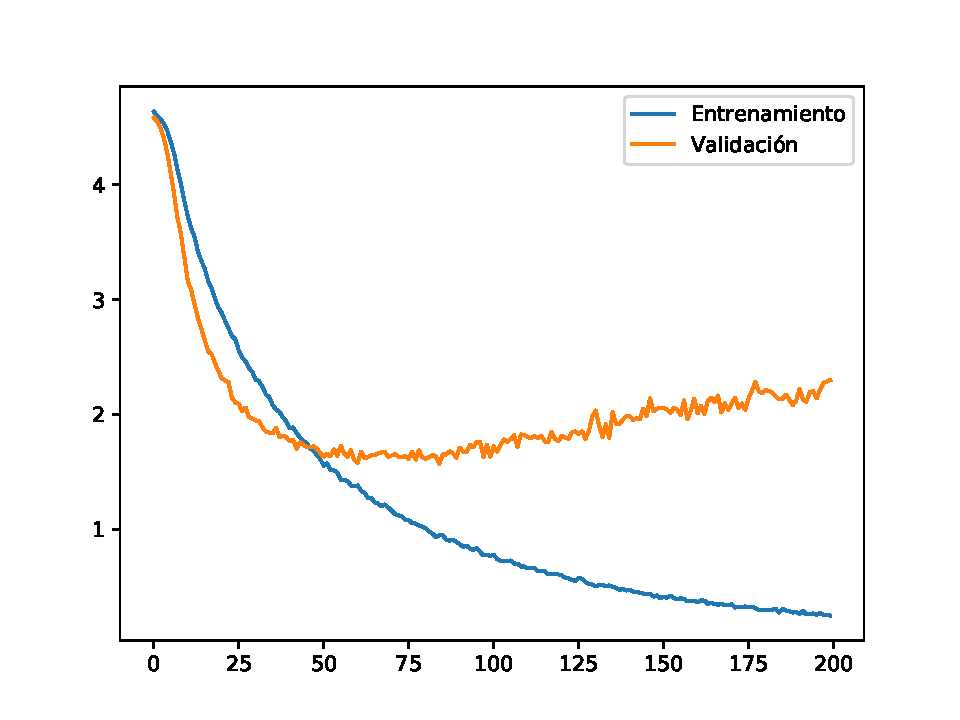
\includegraphics[width=\linewidth]{images/extractor_loss.pdf}
    \caption{Evolución de la función de pérdida.}
  \end{subfigure}
  \begin{subfigure}{0.49\textwidth}
    \centering
    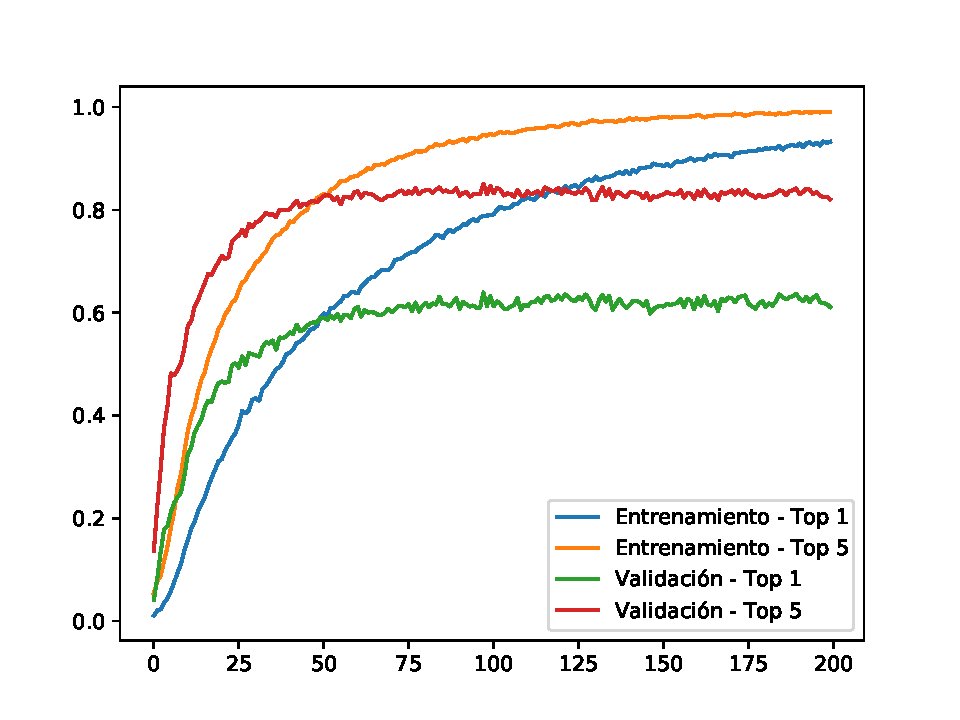
\includegraphics[width=\linewidth]{images/extractor_acc.pdf}
    \caption{Evolución de la precisión Top-1 y Top-5.}
  \end{subfigure}
  \caption{Evolución de la función de pérdida y precisiones para los
    conjuntos de entrenamiento y validación utilizando el extractor
    de características de tamaño 1024.}
  \label{fig:loss-top-k-extractor}
\end{figure}

Gracias al \texttt{ModelCheckpointer} que comentamos previamente,
hemos conservado el estado del modelo en la época 100 para nuestro
extractor de características. Hemos considerado que en dicho punto se
obtiene un modelo de calidad a partir de las métricas que hemos
calculado. En el punto de guardado anterior, a las 80 épocas, el
modelo tiene un comportamiento ligeramente peor en términos de
precisión tanto Top-1 como Top-5, y unos valores de la función de
coste muy similares. El siguiente punto punto de guardado, a las 120
épocas, ya se encuentra en la fase en la que el modelo sobreajusta,
por lo que nos hemos quedado con el modelo intermedio.\\

Tras el entrenamiento de los modelos extractores, obtenemos la siguiente
tabla de precisiones:

\begin{table}[H]
  \centering
  \begin{tabular}{lcc}
    \toprule
    Dimensión del descriptor & Precisión Top-1 & Precisión Top-5 \\
    \midrule
    512 elementos & 57.63 \% & 82.42 \% \\
    768 elementos & 62.98 \% & 84.67 \% \\
    1024 elementos & 63.27 \% & 84.66 \% \\
    \bottomrule
  \end{tabular}
  \caption{Resultados Top-1 y Top-5 de los tres extractores sobre UCF-101}
  \label{tab:extractor-accs}
\end{table}

Como podemos comprobar, para las tres dimensiones obtenemos un modelo
de bastante calidad. El modelo C3D original muestra en su
experimentación \cite[Figura~2]{tran2015learning} que su modelo llega
a una precisión Top-1 de 45 \% cuando se entrena como una red neuronal
completa (al igual que hemos hecho nosotros). Después, muestran los
resultados de su modelo final, que emplea las características de C3D
pero utiliza una SVM para la clasificación final, y cuyos resultados
son significativamente mejores, con una precisión Top-1 de más del 80
\%. No obstante, como estamos interesados en comparar los extractores
de características, creemos que la comparación justa debe ser con el
modelo neuronal completo. Por los resultados obtenidos, podemos
concluir que nuestro extractor es más potente que el que ellos
proponen, al menos en cuanto a clasificación en UCF-101 se refiere.\\

Comparando los resultados de nuestros tres extractores, parece claro
que existe una mejoría cuanto mayor es el tamaño del vector de
características. Dicha mejora no es tan notable entre el extractor de
dimensión 768 y el de tamaño 1024, cuyos resultados son muy similares
(especialmente en términos de precisión Top-5). No obstante, sí que
se observa una mejora sustancial entre estos dos modelos y el más
pequeño.

\subsection{Extracción de características}

Para la extracción de características de los vídeos del conjunto
UCF-Crime, seguimos la misma política que en el trabajo original.
Dividimos el vídeo en fragmentos de 16 fotogramas sin solapamiento,
preprocesamos los fotogramas para llevarlos a tamaño $299 \times 299$,
y utilizamos la función proporcionada por Keras de preprocesado
para Xception.\\

Utilizando la red entrenada según el apartado anterior sin las capas
densas, conseguimos para cada vídeo una representación de tamaño
$k \times 1024$, con $k$ igual al número de fragmentos no solapados de
16 fotogramas. Agrupando dichos fragmentos en 32 grupos y tomando la
media de los fragmentos de cada grupo, obtenemos la representación
final del vídeo formada por 32 fragmentos, cada uno de ellos con un
vector de características de tamaño 1024.

\subsection{Entrenamiento del clasificador}

Una vez tenemos las características extraídas, aplicamos una
estrategia análoga a la del modelo original para el entrenamiento del
clasificador. El clasificador es de nuevo una red neuronal
completamente conectada, pero de tamaño menor a la empleada por el
modelo original. Tenemos dos capas ocultas, de tamaño 512 y 64,
respectivamente, y la neurona de salida. La disminución del tamaño de
las capas ocultas viene justificada por la reducción del tamaño del
descriptor, que ha pasado a tener la mitad del tamaño original.\\

Además, se ha reducido la tasa de desactivación de las capas de
\textit{Dropout} de 0.6 a 0.4, ya que hemos considerado que en el
modelo original se tomaba un valor excesivo, el cual puede hacer
también que el rendimiento del clasificador se degrade y el
entrenamiento sea mucho más lento.\\

Se han ajustado también los valores de ponderación de los términos de
la función de pérdida. Se ha aumentado el valor el regularizador del
núcleo a 0.01, y se han reducido los multiplicadores de las
restricciones temporales y dispersas a la mitad (de 0.00008 a
0.00004). Estos ajustes se han hecho tras estudiar los primeros
entrenamientos del modelo y observar que cometía demasiados falsos
negativos. Esto podía ocurrir porque las restricciones de dispersión
fuesen demasiado fuertes, así que hemos mitigado ligeramente ese
efecto reduciendo la importancia del término.\\

El optimizador utilizado en nuestro caso es de nuevo Adagrad, aunque
hemos aumentado la tasa de aprendizaje a 0.2 al principio. Se ha
observado que el entrenamiento es bastante lento al principio, y esta
modificación mejora este mal comportamiento inicial.

\section{Resultados obtenidos}

En esta sección, mostramos los resultados obtenidos en el experimento
final. En primer lugar, mostramos las matrices de confusión para el
umbral de decisión 0.5 de ambos modelos:

\begin{table}[H]
  \centering
  \begin{tabular}{lcccc}
    \toprule
    Modelo & TN & FP & FN & TP \\
    \midrule
    Original - preentrenado & 902433 & 125044 & 49699 & 34632 \\
    Original - replicado & 783342 & 244135 & 43699 & 40632 \\
    Xception-LSTM - 1024 & 875515 & 151962 & 44145 & 40186 \\
    Xception-LSTM - 768 & 908518 & 118959 & 52874 & 31457 \\
    Xception-LSTM - 512 & 914259 & 113218 & 60661 & 23670 \\
    \bottomrule
  \end{tabular}
  \caption{Matrices de confusión para los modelos entrenados}
  \label{tab:confusion-matrices}
\end{table}

En la tabla podemos observar varios detalles que merece la pena
comentar. En primer lugar, podemos observar cómo el modelo original
entrenado por los autores (marcado aquí como preentrenado) y el modelo
original replicado por nosotros no obtienen resultados
equivalentes. Nuestra réplica consigue un mayor número de verdaderos
positivos, con un aumento de 6000 fotogramas anómalos detectados, pero
a cambio de aumentar significativamente el número de falsos
positivos. Este es el motivo por el que hemos decidido replicar la
experimentación, ya que normalmente es muy difícil replicar las
condiciones de entrenamiento de un modelo, y por tanto la comparativa
con los resultados originales puede no ser del todo justa. El modelo
replicado por nosotros ha sido entrenado en unas condiciones similares
a las que hemos impuesto a nuestra propuesta, por lo que la
comparativa es, desde nuestro punto de vista, más justa con dicho
modelo.\\

Comparando nuestras propuestas entre sí, podemos observar cómo el
tamaño de la representación afecta significativamente a los resultados
que obtiene el modelo. Cuanto mayor es el vector de características,
más fotogramas anómalos se detectan, a costa de cometer también más
falsos positivos. No obstante, el aumento de falsos positivos no es
tan notable como el aumento de fotogramas bien clasificados, por lo
que consideramos que nuestro modelo mejora con el aumento del tamaño
de la representación.\\

Resulta especialmente notable comparar el aumento de falsos positivos
entre los modelos. Mientras que para los modelos de 512 y 768
características, el aumento de falsos positivos es pequeño (de hecho,
en términos absolutos, el aumento de falsos positivos es menor que el
aumento de verdaderos positivos, a pesar del desbalanceo de clases),
cuando observamos el modelo de tamaño 1024 este problema se
dispara. Convendría estudiar por qué se ha producido dicho aumento.\\

En cuanto a la comparativa entre nuestra propuesta y el modelo
original, si nos comparamos con nuestra experimentación, el modelo
propuesto de mayor tamaño de representación es significativamente
mejor que la propuesta original. El número de verdaderos positivos es
prácticamente el mismo, pero el número de falsos positivos se ha
reducido drásticamente. Esto indica que las características que hemos
extraído permiten diferenciar mejor los fotogramas normales de los
anómalos que las que extrae el modelo C3D. Si nos comparamos con la
propuesta original entrenada por los autores originales, obtenemos un
aumento considerable en el número de verdaderos positivos (detectamos
unos 6000 fotogramas positivos más), pero a costa de un aumento
también significativo de falsos positivos. En este caso,
probablemente, la decisión entre escoger un modelo u otro si nos
fijamos exclusivamente en las matrices de confusión vendría
justificada por los requerimientos del problema real a resolver.  En
este caso, el detectar un mayor número de positivos es recomendable,
ya que estamos hablando de un sistema de alarma.  Cometer un falso
positivo será menos grave que cometer un falso negativo, ya que en el
caso de falso positivo simplemente se avisa de algo que en realidad no
está ocurriendo, pero en el caso del falso positivo podemos ignorar
una situación de peligro que sí interesaría detectar.\\

Además de las matrices de confusión, mostramos a continuación las
curvas ROC y las curvas PR:

\begin{figure}[H]
  \centering
  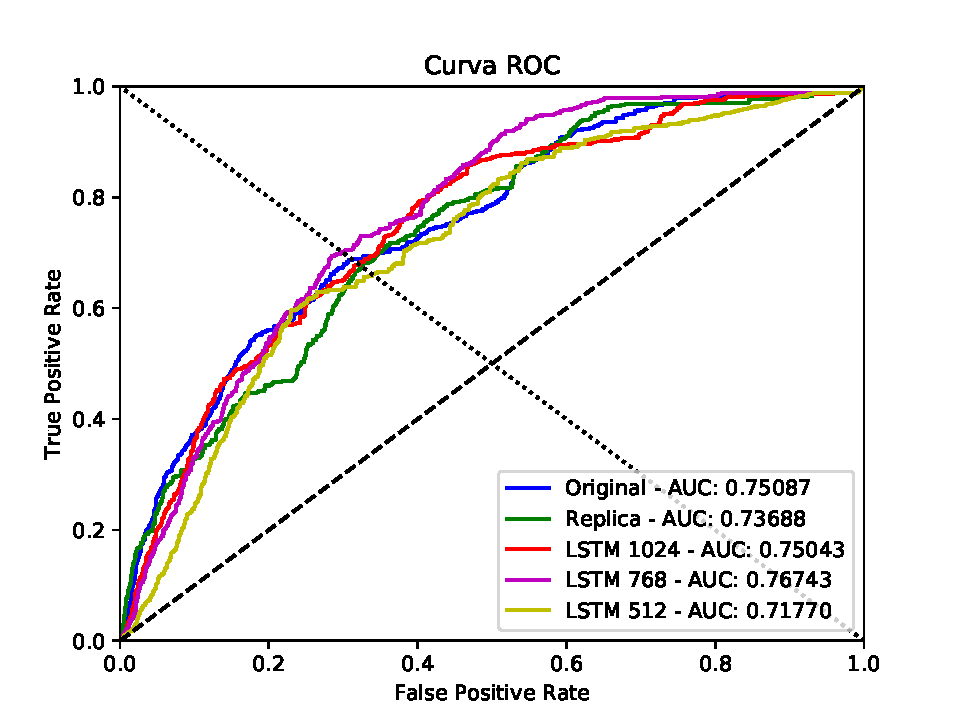
\includegraphics[width=.8\textwidth]{images/roc_overlay.pdf}
  \caption{Curvas ROC de los modelos}
  \label{fig:roc-curves-experiments}
\end{figure}

A la vista de las curvas ROC, podemos concluir que todos los modelos
tienen un comportamiento similar. En principio, los dos modelos de
peor calidad en cuanto a la curva ROC se refiere son la réplica del
modelo original y el modelo Xception-LSTM con tamaño de 512
características.  Estas dos curvas son dominadas por las otras 3
prácticamente en todo el gráfico. Por otro lado, la curva obtenida por
el modelo Xception-LSTM de tamaño 768 es claramente la dominante en
gran parte del gráfico. Para tasas bajas de falsos positivos dicha
ventaja no es tan notable, pero rápidamente pasa a ser el mejor modelo
y domina al resto de curvas en el resto del gráfico, alcanzada
sólamente por la representación de 1024 elementos para una tasa de
falsos positivos en torno al 0.4.\\

Otro detalle que podemos observar es que los modelos basados en
convolución exclusivamente tienen mejor comportamiento que nuestros
modelos cuando hablamos de tasas bajas de falsos positivos. Tanto el
modelo original como la réplica se mantienen como mejores modelos
cuando hablamos de una tasa de falsos positivos por debajo de 0.1. No
obstante, a partir de ese punto, nuestras propuestas alcanzan un
rendimiento similar a las propuestas originales, y las superan
rápidamente para el resto del gráfico.\\

Si nos fijamos en términos de AUC, sorprendentemente el mejor modelo
encontrado es el que utiliza la representación de tamaño 768. Aunque
en la matriz de confusión nos pareció mejor el modelo de tamaño 1024,
en términos de AUC tenemos un mejor comportamiento por parte del
modelo de tamaño medio. En particular, supera por más de 1.5 puntos
porcentuales tanto al modelo original como a nuestra propuesta de
mayor tamaño, los cuales consiguen unos resultados muy
similares. Estamos hablando de una mejora relativamente amplia, por lo
que este modelo podría ser el más adecuado en algunos
contextos. Además, el EER, que es el punto en el que la curva ROC se
corta con la línea de puntos diagonal, muestra también que el mejor
modelo es la LSTM de tamaño 768. A continuación, con un resultado muy
similar entre ellas, están las dos convolucionales completas y el
modelo LSTM de tamaño 1024. Finalmente, el modelo que peor
comportamiento tiene en este caso es de nuevo la LSTM
de tamaño 512.\\

Pasamos a mostrar las curvas PR:

\begin{figure}[H]
  \centering
  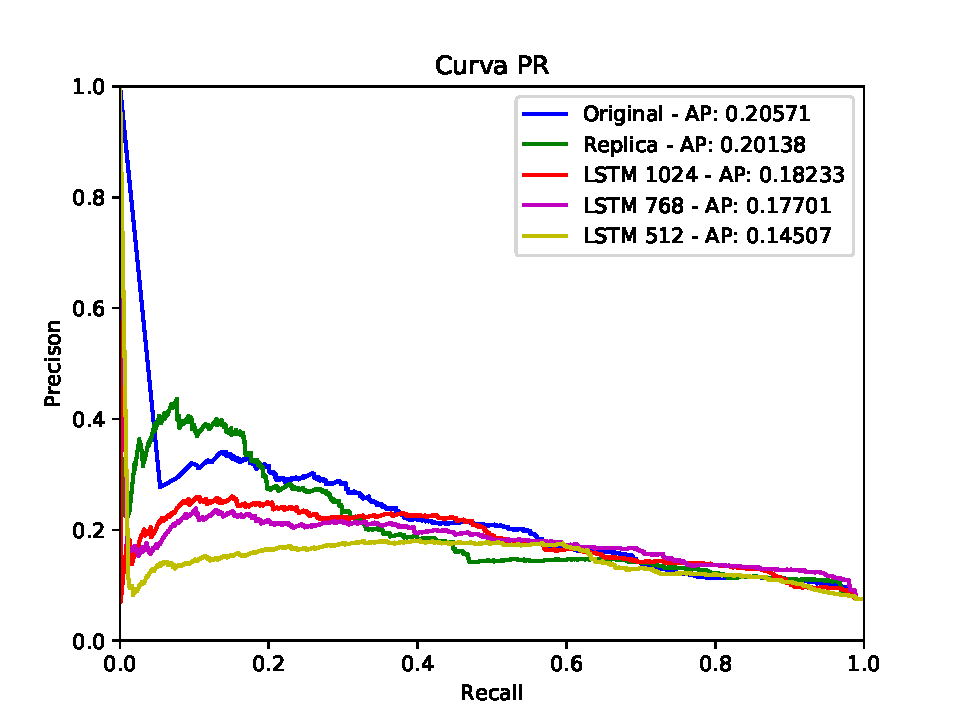
\includegraphics[width=.8\textwidth]{images/pr_overlay.pdf}
  \caption{Curvas PR de los modelos}
  \label{fig:pr-curves-experiments}
\end{figure}

En esta comparativa encontramos resultados muy dispares. Por un lado,
si nos fijamos en la parte izquierda de la gráfica, tenemos que la
réplica del modelo original es la que mayor precisión tiene, pero ahí
estamos hablando de tasas de verdaderos positivos bajas (esta métrica
recibe en inglés el nombre de \textit{Recall}, y es el nombre que se
muestra aquí). También tenemos por encima en este caso al modelo
original. Conforme vamos avanzando por el gráfico hacia niveles
mayores de \textit{recall}, la réplica pasa a perder mucha precisión,
y rápidamente se convierte en el peor de los modelos. Algo similar le
ocurre al modelo original, el cual acaba siendo superado por el modelo
de tamaño 1024 y el de tamaño 768. No obstante, la pérdida de
rendimiento en este caso es mucho más gradual que en la réplica.\\

Nuestros tres modelos, por el contrario, tienen un comportamiento
similar durante todo el gráfico. Aunque no llegan a tener niveles de
precisión muy altos en ningún punto, sí que se mantiene la misma de
forma más o menos constante. Llegan a superar a los modelos originales
en una gran parte del gráfico. No obstante, debido al buen rendimiento
del modelo convolucional en tasas bajas de verdaderos positivos,
cuando miramos la precisión media tanto el original como la réplica
quedan por encima de todas nuestras propuestas.\\

Este buen comportamiento al principio significa que los modelos
convolucionales consiguen diferenciar más claramente los
comportamientos claramente anómalos que los modelos Xception-LSTM. Es
decir, para aquellos ejemplos en los que es clara la anomalía, el
modelo convolucional suele responder de forma más segura, por lo que
clasifica correctamente un porcentaje importante de fotogramas de este
tipo. Por otro lado, cuando empiezan a aparecer fotogramas de
clasificación más difícil, los modelos Xception-LSTM pasan a
comportarse mejor que los modelos convolucionales puros.\\

Pasamos a mostrar y analizar la tabla de métricas comparativas:

\begin{table}[H]
  \centering
  \begin{tabular}{lccccc}
    \toprule
    Modelo & Exactitud & AUC & $F_1$ & EER & AP \\
    \midrule
    Original - preentrenado & 0.8428 & 0.7508 & 0.2838 & 0.3119 & \textbf{0.2057} \\
    Original - replicado & 0.7411 & 0.7369 & 0.2201 & 0.3253 & 0.2014 \\
    Xception-LSTM - 1024 & 0.8236 & 0.7504 & \textbf{0.2907} & 0.3221 & 0.1823 \\
    Xception-LSTM - 768 & \textbf{0.8455} & \textbf{0.7674} & 0.2681 & \textbf{0.2980} & 0.1770 \\
    Xception-LSTM - 512 & 0.8436 & 0.7177 & 0.2140 & 0.3388 & 0.1451 \\
    \bottomrule
  \end{tabular}
  \caption{Tabla de métricas comparativas de los modelos a nivel de fotograma}
  \label{tab:confusion-matrices}
\end{table}

La primera métrica con la que nos encontramos es la exactitud. Aunque
sabemos que esta métrica es poco relevante cuando nos encontramos ante
un problema de clasificación muy desbalanceado, como el nuestro, es
una métrica que se calcula normalmente, por lo que hemos decidido
incluirla. Para esta métrica, tenemos el mejor comportamiento para el
modelo LSTM de tamaño 768, aunque casi todos los modelos obtienen unos
resultados similares. El modelo original replicado es claramente el
peor de los cinco en esta métrica, el cual obtiene unos 10 puntos
porcentuales menos que el resto.\\

En términos de AUC, como ya habíamos visto en la gráfica anterior, el
mejor modelo es la propuesta de tamaño 768, que supera ampliamente al
resto de modelos. En particular, obtiene mejores resultados que el
propio modelo original en el artículo, lo cual abre la puerta a una
posible publicación tras un estudio más exhaustivo. Es importante
remarcar que nuestro extractor fue preentrenado en un conjunto que
contiene menos información que el utilizado en el extractor original,
por lo que este margen de mejora que hemos obtenido podría agrandarse
más con los nuevos datos. En cuanto al resto de modelos, podemos
observar cómo el modelo original consigue un resultado similar al
obtenido por la propuesta de tamaño 1024. Ligeramente por debajo queda
el modelo réplica, y por último el modelo de Xception-LSTM de tamaño 512.\\

La mejora que consideramos más importante derivada de nuestro estudio
se produce sobre la métrica $F_1$ para el umbral de decisión 0.5. Esta
mejora era previsible teniendo en cuenta los resultados que observamos
sobre la matriz de confusión, pero aquí confirmamos que efectivamente
se produce. En particular, hemos mejorado esta métrica con el modelo
propuesto de tamaño 1024, que consigue la puntuación más alta de todos
los modelos. Consideramos esta métrica especialmente relevante porque
representa el comportamiento que tiene nuestro modelo respecto a la
clase positiva, que es en la que más interesados estamos. Esto implica
que, para el umbral de decisión fijado, el modelo Xception-LSTM de
mayor tamaño se comporta mejor que el modelo original, lo cual apoya
la hipótesis que teníamos de partida. Resulta curioso observar que, a
pesar de ser el mejor modelo en términos de AUC por un margen
importante, el modelo de dimensión 768 obtiene peores resultados
en esta métrica. Esto pone de manifiesto la importancia de utilizar
diversas métricas para comparar modelos, ya que el uso de una única
medida, a no ser que estemos muy
interesados en un comportamiento concreto, suele dar ideas erróneas.\\

Las dos últimas métricas que mostramos hemos podido observarlas
previamente en las gráficas mostradas. La tasa de error igual (EER),
la cual indica un mejor modelo cuanto menor sea el valor, pudimos
observarla en la gráfica de las curvas ROC, ya que es el punto en el
que se cruzaban las curvas con la diagonal de puntos. Como ya dijimos,
el modelo de dimensión 768 es el mejor modelo en términos de esta
métrica. El AP, que se mostraba en la leyenda de la gráfica PR, nos
dice que los mejores modelos en términos de precisión media son los
modelos convolucionales puros, debido a la precisión tan alta que
tenían para las tasas de acierto bajas.\\

Por último, mostramos los resultados en términos de capacidad de
clasificación de los modelos a nivel de vídeo. La capacidad de los
modelos de detectar la presencia de una anomalía puede ser incluso más
importante que la localización exacta de dicha anomalía dentro del
vídeo. Aunque la anomalía no esté perfectamente delimitada, es decir,
que los primeros o últimos segundos de la anomalía no queden
precisamente delimitados, el hecho de generar la alarma cuando
efectivamente se produce una situación anómala, y no hacerlo cuando
nos encontramos ante un vídeo normal, es de gran importancia si se
pretende implementar un sistema de estas características en un
entorno real.\\

En la siguiente tabla se pueden observar los resultados de los modelos
en términos de evaluación a nivel de vídeo:

\begin{table}[H]
  \centering
  \begin{tabular}{lcc}
    \toprule
    Modelo & \% Vídeos normales  & \% Vídeos anómalos \\
    \midrule
    Original & 13.33 & 64.89 \\
    Réplica & 11.11 & 74.05 \\
    Xception-LSTM - 1024 & 15.55 & \textbf{77.86} \\
    Xception-LSTM - 768 & 12.59 & 72.52 \\
    Xception-LSTM - 512 & \textbf{8.15} & 71.76 \\
    \bottomrule
  \end{tabular}
  \caption{Porcentaje de vídeos normales y anómalos en los que se ha
    generado una alarma. Para los vídeos normales, un porcentaje mayor
    implica que se han generado más falsas alarmas en vídeos normales,
    y por tanto un peor rendimiento del modelo. Para los vídeos
    anómalos, por el contrario, un porcentaje más alto indica indica
    que se han detectado anomalías en un número mayor de vídeos, y por
    tanto mejores resultados.}
  \label{tab:video-level-predictions}
\end{table}

Para estas métricas, podemos observar que nuestra propuesta es también
de bastante calidad. Por un lado, se observa que el modelo original
tiene un comportamiento bastante mejorable, especialmente en términos
de vídeos anómalos sin etiqueta. En particular, no se generan alarmas
en uno de cada tres vídeos, lo que significa que es un modelo bastante
poco fiable para su uso en entornos reales. El modelo original
replicado por nosotros mejora notablemente estos resultados, generando
un menor número de alarmas en vídeos normales, y un aumento
significativo de alarmas para vídeos anómalos. Concretamente, sólo se
pierden alarmas en uno de cada cuatro vídeos. Sigue siendo un valor
alto, pero significativamente mejor que el original.\\

Comparando entre si los resultados obtenidos por nuestros modelos,
tenemos que cuanto mayor es el tamaño de representación, más
información de anomalía se recoge. El aumento del tamaño del
descriptor lleva acompañado un aumento importante del número de vídeos
positivos en los que se genera una alarma. Como contrapartida, también
se cometen un número mucho mayor de falsos positivos. Es especialmente
notable el mal comportamiento del modelo de 768 características en
este caso. Apenas mejora el porcentaje de vídeos detectados respecto
al modelo de tamaño 512, y por otro lado comete casi tantas falsas
alarmas como el modelo de tamaño 1024.\\

Entre el modelo de tamaño 1024 y el modelo original entrenado por
nosotros, que son los dos que mejores resultados obtienen, la decisión
entre cuál tiene mejor comportamiento es subjetiva. Nuestro modelo es
capaz de detectar un mayor número de vídeos anómalos, pero a cambio de
un aumento en el número de falsas alarmas importante. Probablemente,
si el modelo va a utilizarse en una aplicación real, estaremos más
interesados en un modelo similar al nuestro, ya que interesará
detectar el mayor número de situaciones anómalas posible. El hecho de
que ocurran falsos negativos es menos preocupante, ya que una alarma
de este tipo servirá, probablemente, como método de aviso y no como
toma de decisiones. Nos interesa, por tanto, que sea muy sensible
a la clase positiva, y no tanto a la clase negativa, ya que las falsas
alarmas van a ser procesadas a posteriori por un humano.\\

\end{document}

%%% Local Variables:
%%% mode: latex
%%% TeX-master: "../main"
%%% End:
